\subsection{Definition}

The aim of this example is to simulate the stationary groundwater flow in an anisotropic porous medium. In order to consider the permeability anisotropy, a 2-D numerical model is built which contains a higher permeability in the vertical direction than that in the horizontal direction. The aquifer is assumed saturated and stationary.


For the two-dimensional simulation, the cube consisting of a porous medium is simplified as a square with an area of 1~m$^2$. The calculation model includes 736 triangular elements and 409 nodes. At the lower left corner of the model a constant pressure of 1000~Pa is specified along two polylines of the length of 0.3~m (Fig. \ref{GW:anisrotropic}). At the top and the right borders the pressures are set to 0 in order to create the pressure gradient. As the porous medium is assumed to be anisotropic, which influences the groundwater flow, the values for the permeabilities are equal to 1.0$\times 10^{-15}$ m$^2$ in x-direction and 1.0$\times 10^{-14}$ m$^2$ in y-direction. Other property of the anisotropic media is shown in Table. \ref{tab22}. 

\begin{table}[h!]
\centering
\caption{The parameters defined in the anisotropic media.}
\begin{tabular*}{0.9\textwidth}{@{\extracolsep{\fill}}llrr}
\hline\noalign{\smallskip}
 Symbol &Parameter& Value & Unit \\ 
\hline\noalign{\smallskip}
$n$ 				&porosity  		& 0.2 									&  --  \\			
$\kappa_x$ 	&permeability & $1.0\times 10^{-15}$  & $m^2$ \\
$\kappa_y$ 	&permeability & $1.0\times 10^{-14}$ 	& $m^2$ \\
\noalign{\smallskip}\hline
\end{tabular*}
\label{tab22}
\end{table}

\begin{figure}[h!]
\centering
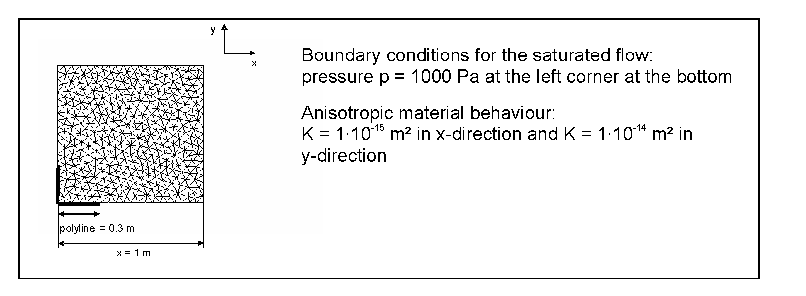
\includegraphics[width=1.0\textwidth]{Chapter5/figure/anisotropicdomain.eps}
\caption{Calculation model (2-D) of the anisotropic media.}
\label{GW:anisrotropic}
\end{figure}

\subsection{Evaluation method}
This test example is not made up to introduce a new process, but it shows the possibility for the OGS user to give a specific permeability for each direction. Therefore, the interpretation of OGS results comprises merely the comparison between pressure distributions due to the anisotropic permeability that were simulated by the use of RockFlow (RF) and OGS. This comparison is possible because both versions are developed separately concerning anisotropy of soils.

\begin{figure}[h!]
\centering
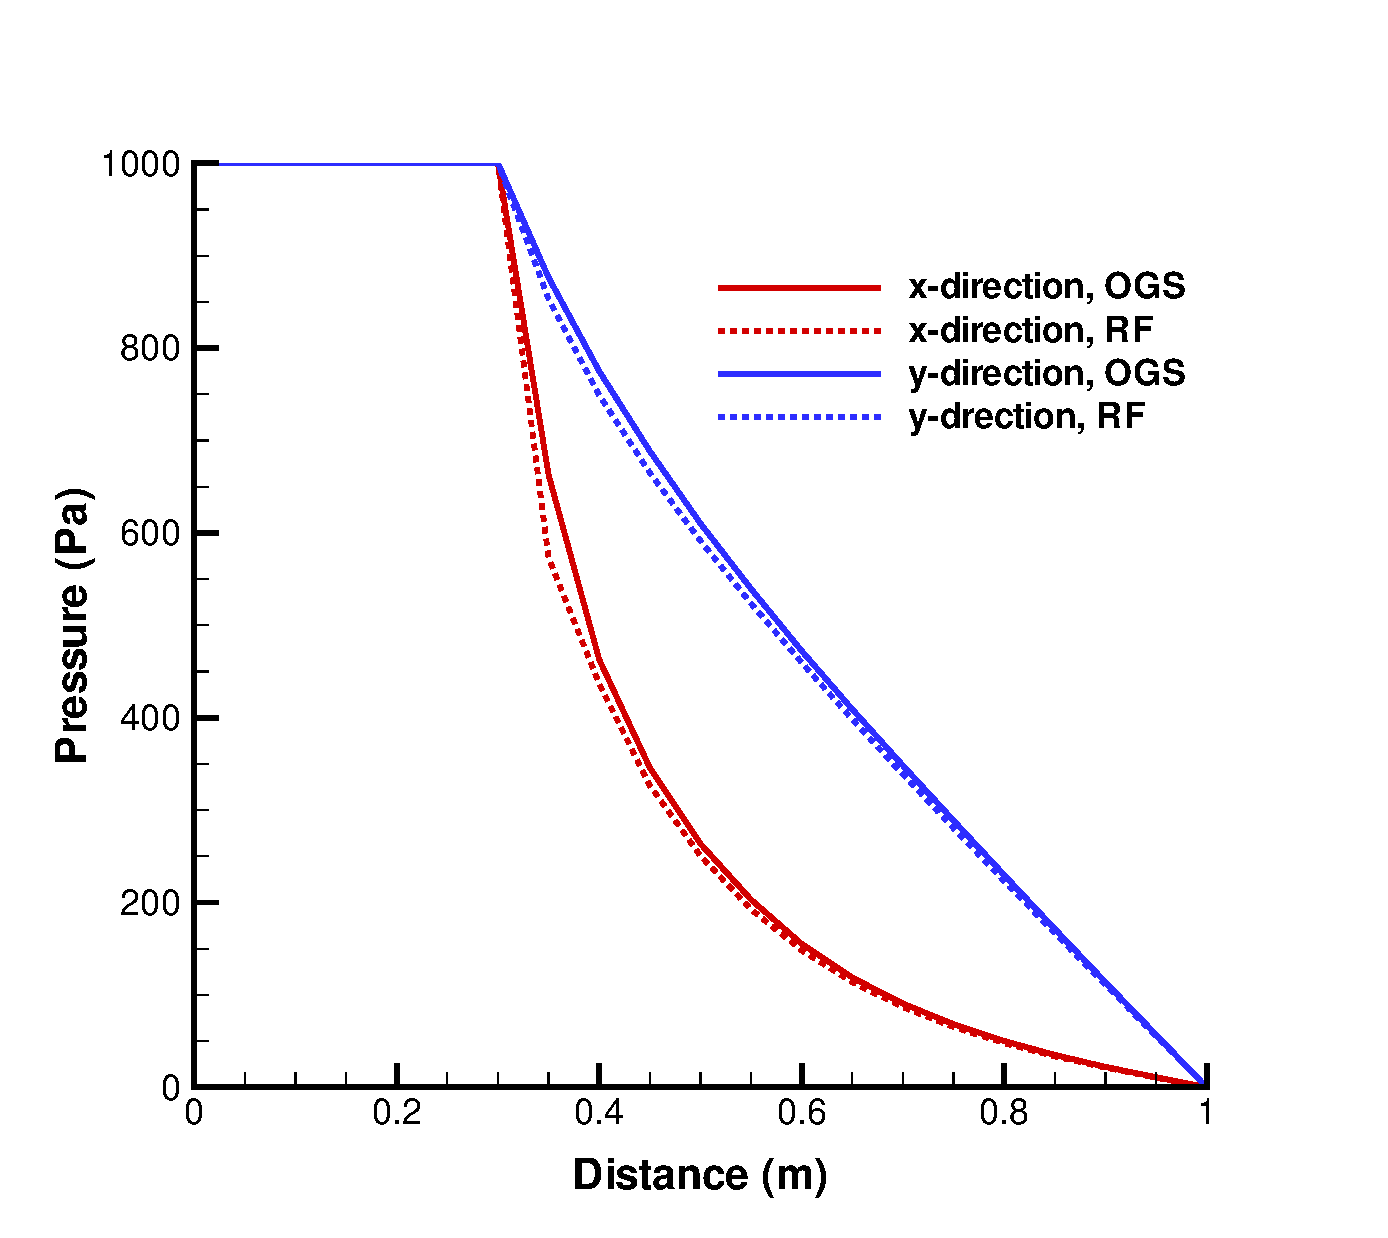
\includegraphics[width=0.6\textwidth]{Chapter5/figure/anisotropicresult.eps}
\caption{Pressure distribution caused by anisotropic saturated flow.}
\label{GW:anisotropicresult}
\end{figure}

\subsection{Results}

In Fig. \ref{GW:anisotropicresult} the horizontal and vertical pressure distributions of an anisotropic groundwater flow model which is developed using the program code RF are depicted next to those calculated from the above described anisotropic model with OGS. While presuming an anisotropic medium, an inhomogeneous pressure field is developing because the groundwater is not able to spread out uniformly. This can be recognized at the different curve gradients in x- and y-direction. There are slight differences between the curve characteristics of the RF and OGS simulation results. These differences are due to different element types (square in the RF model) and the resulting different x- or y-coordinates. Therefore, the pressure distributions obtained by the simulation with OGS are evaluated to be correct.